% tex file for convolution
\subsubsection{Convolution}
\par \indent Our study is structured around event-related neurological 
stimulus, rather than block stimulus, as was the case of the data used in 
class examples. So, we could not repurpose the class approach for 
representing the hemodynamic response to our analysis. 

\par It is assumed that there is a relationship between the hemodynamic 
response to the neurological stimuli. Further, there is the assumption that 
a single stimulus generates a delayed hemodynamic response that mirrors a 
double-gamma function, and that multiple stimuli have an additive nature, as 
defined below: 

\begin{equation} \label{eq:convolve}
r(t)= \sum_{i=1}^n \psi_{i} \phi_{i}(t-t_i)
\end{equation}

\noindent where $\psi_i$ is the amplitude of the response stimulus (assumed to 
be always $1$ in our case), and $\phi_{i}$ is the hemodynamic response started 
at the $i$th stimulation ($t_i$).

\par We attempted five approaches that can each be grouped into one of three 
subcategories: \textbf{(1)} a strict replication of equation 
\ref{eq:convolve}; \textbf{(2)} a matrix multiplication equivalent to 
\textbf{(1)}; and \textbf{(3)} a complex function that takes advantage of the 
speed of \texttt{np.convolve}. This complicated function first splits the 
(two-second)intervals between each scan into a given number of even slices, 
then puts the stimulus into the closest slice with respect to time, and 
finally calls \texttt{np.convolve} on this much longer time series and a 
detailed hrf function, before reducing back down to the dimensions of the 
original scan time series at two-second intervals. Detailed exploration of 
this matter can be found in Appendix \ref{app_convolution}.

We compared these methods based on accuracy and speed. Figure 
\ref{fig:convolution_a} displays an accuracy comparison, and 
Table~\ref{fig:convolution_a} shows the accuracy based off of 
\texttt{ipython}'s \%\texttt{timeit} magic command.



\begin{figure}[ht]
\centering
	\begin{minipage}[b]{0.45\linewidth}
		\centering
		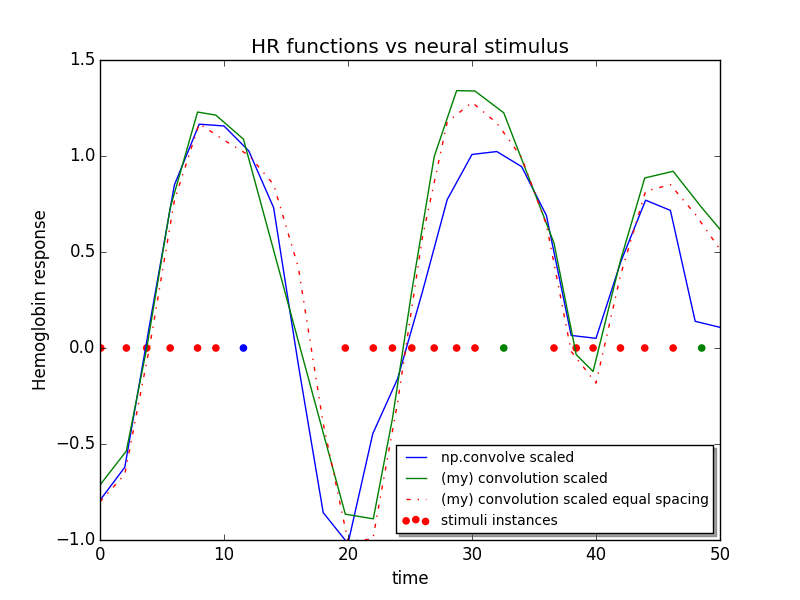
\includegraphics[width=.8\linewidth]{../images/convolution_vs_neural_stimulus}
		% needs to be from the event_related_HRF_script2.py 
		\caption{\scriptsize{Different convolution functions vs. the Neural stimulus}}
		\label{fig:convolution_a}

	\end{minipage}
\quad
	\begin{minipage}[b]{0.45\linewidth}
		\centering
		\begin{tabular}{|l | c|}
		\hline
		name in graph       & Speed per loop \\
		\hline
		np naive approach & 14.4 $\mu$s  \\
		user 2     		    & 972 ms  \\
		user 3     		    & 1.15 s    \\
		user 4 (15 cuts)      & 98.3 ms \\
		user 4 (30 cuts)      & 185 ms  \\
		user 5     	 	    & 110 ms   \\
		\hline
		\end{tabular}
		\vspace{5mm}
		\label{tab:convolution_a}
		\captionof{table}{\scriptsize{Speed to create HRF predictions for 
		Subject 001, all conditions}}
	\end{minipage}
\end{figure}

\par \noindent The first method in the table, ``np naive approach'', blindly 
plugs our data into the \texttt{np.convolve} function. It is provided to 
showcase potential speed. The failure of the "np naive approach" was the 
motivating factor behind the rest of the hemodynamic response convolution 
analysis, due to a lack of equidistant spacing of stimulus and scans. The 
``user 2'' and ``user 3'' functions runs fall under subcategory 
\textbf{(1)}. ``user 2'' was the first approach to
match the theory, but it matches the stimulation times and not the scan times.
``user 3'' is the most theoretically sound model (and is our standard for 
accuracy). The ``user 5'' falls under subcategory \textbf{(2)}, ``User 5''  is
our matrix version of the theory, and has the same accuracy as ``user 3''. The 
``user 4'' models falls under subcategory \textbf{(3)}, the methods that use the
grid cut usage of \texttt{np.convolve} with notations for the number of slices 
between each scan. We concluded that "user 4 (15 cuts)" was the best approach 
since it gives us speed and very close accuracy to the golden standard - ``user 
3".

\subsubsection{Time Correction}

\par \indent The fMRI machine scans each voxel at a slightly different time. 
In our case, the lowest horizontal slice was scanned first, with the later 
scans obtained in order progressively toward the top of the brain. The signs 
of this linear change in time of scan was observed when running simple 
regression on the data and found that the hemodyamic response $\hat{\beta}$ 
values from all conditions grouped together. We corrected for the time 
differences by shifting the times of stimuli ``backwards'' for voxels scanned 
later to directly correct for the delay of the scan (assuming that each layer 
of the scan took 2/34 of a second).

\subsubsection{Multiple Conditions}

\par \indent Originally, we used multiple regression to acount for the 
three different types of stimulus (pump, explode, cash-out) and examine if the 
separation of these stimuli can better describe the response. We did this by 
creating separate predicted hemodynamic reponses for each condition to allow 
for different amplitudes for each type of condition. As will be noted in 
Section \ref{model_selection} portion later, we did not observe a large 
difference in the results values we obtained, so we did not continue with 
this exploration. In Figure \ref{fig:all_cond_time}, we can see the different 
conditions separated the responses for each condition.
 

\begin{figure}[ht]
\centering
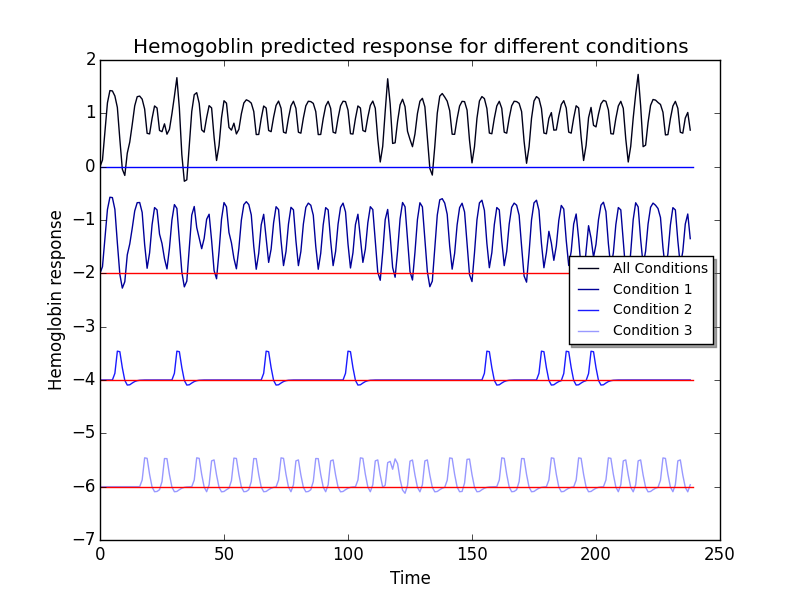
\includegraphics[scale=.5]{../images/all_cond_time}  
\caption{Plotting all predicted HR for conditions.}
\label{fig:all_cond_time}
\end{figure}

A more detailed discussion about our approach and the theory behind convolution 
of the hemodynamic response with the neurological response can be found 
in Appendix \ref{app_convolution}.

